\section{}
\label{prototype:DocumentTagging}

Alongside the ability to visually create tags through dragging edges between nodes in the graph view, I have also implemented a 'tagbar' underneath the document title. Once a user clicks on the tabbar they can begin typing a pre-existing tag to add it to the note or simpply create a new tag from the very same input. In a similar way users can also remove tags by selecting them as they are added from the tagbar.

\begin{figure}[H]
    \centering
    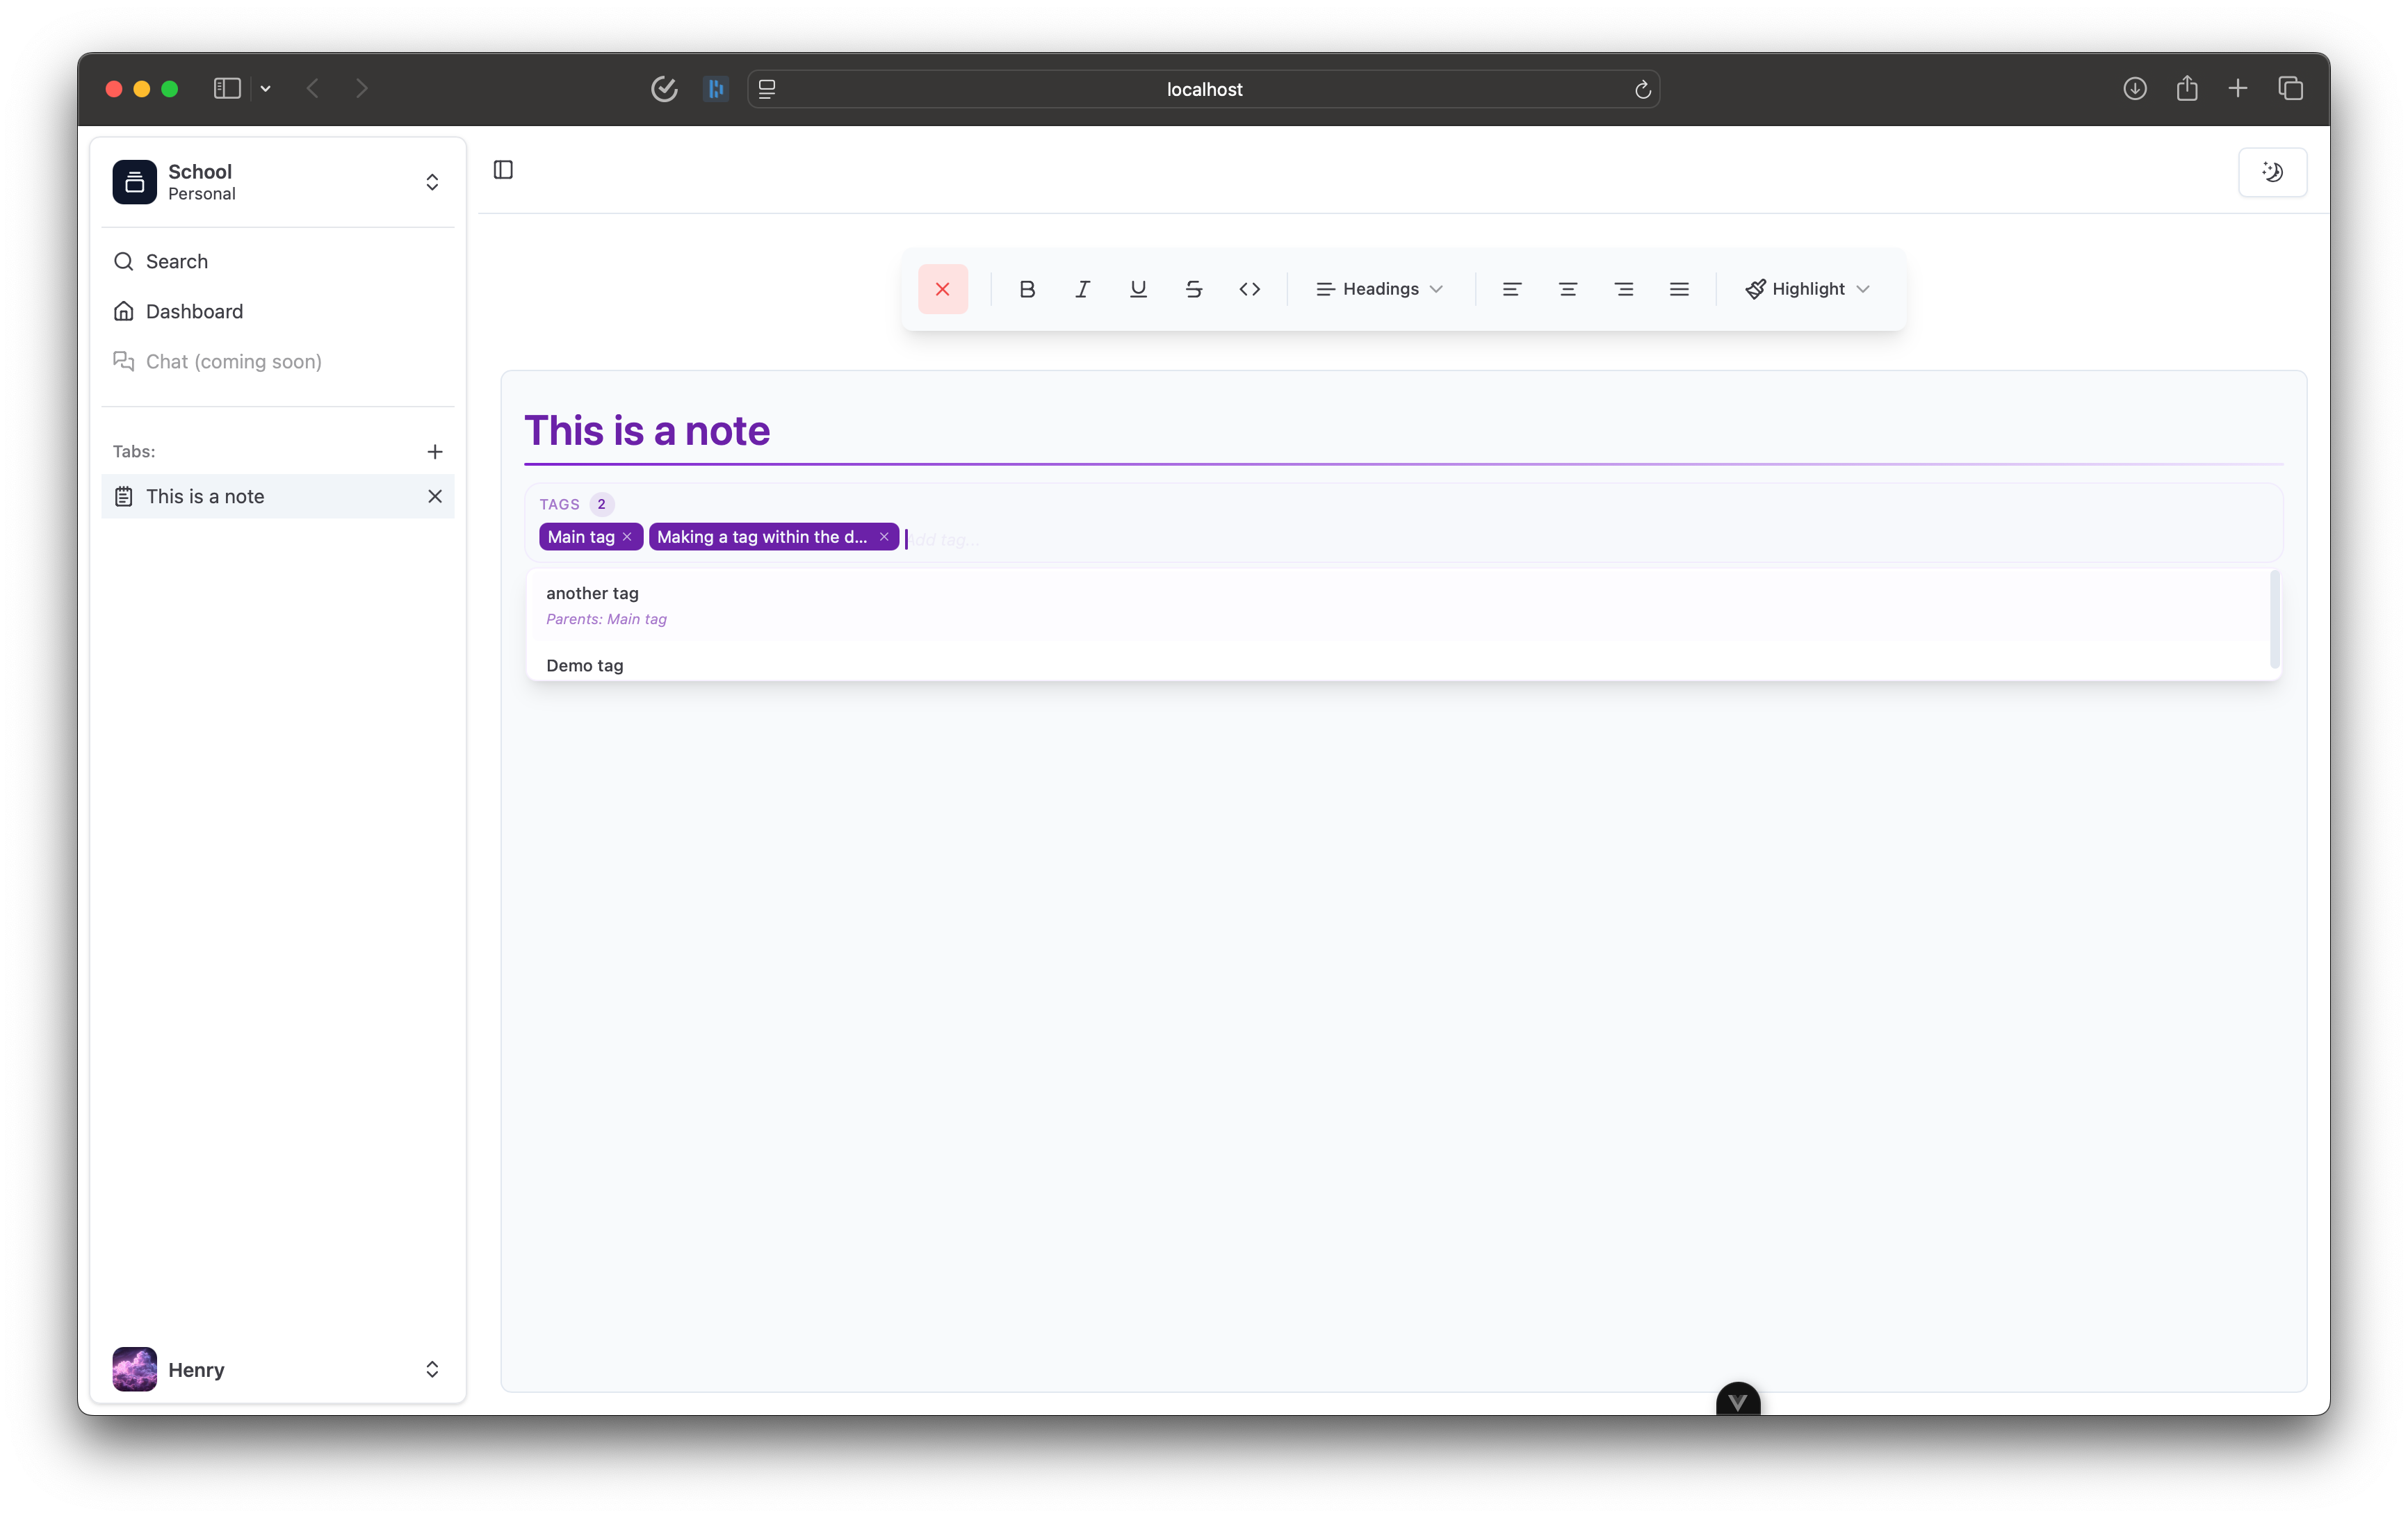
\includegraphics[width=0.8\textwidth]{Prototype/23_DocumentTagging/media/addingTag.png}
    \caption{Attaching a tag to a document}
    \label{fig:document_tagging}
\end{figure}

\begin{figure}[H]
    \centering
    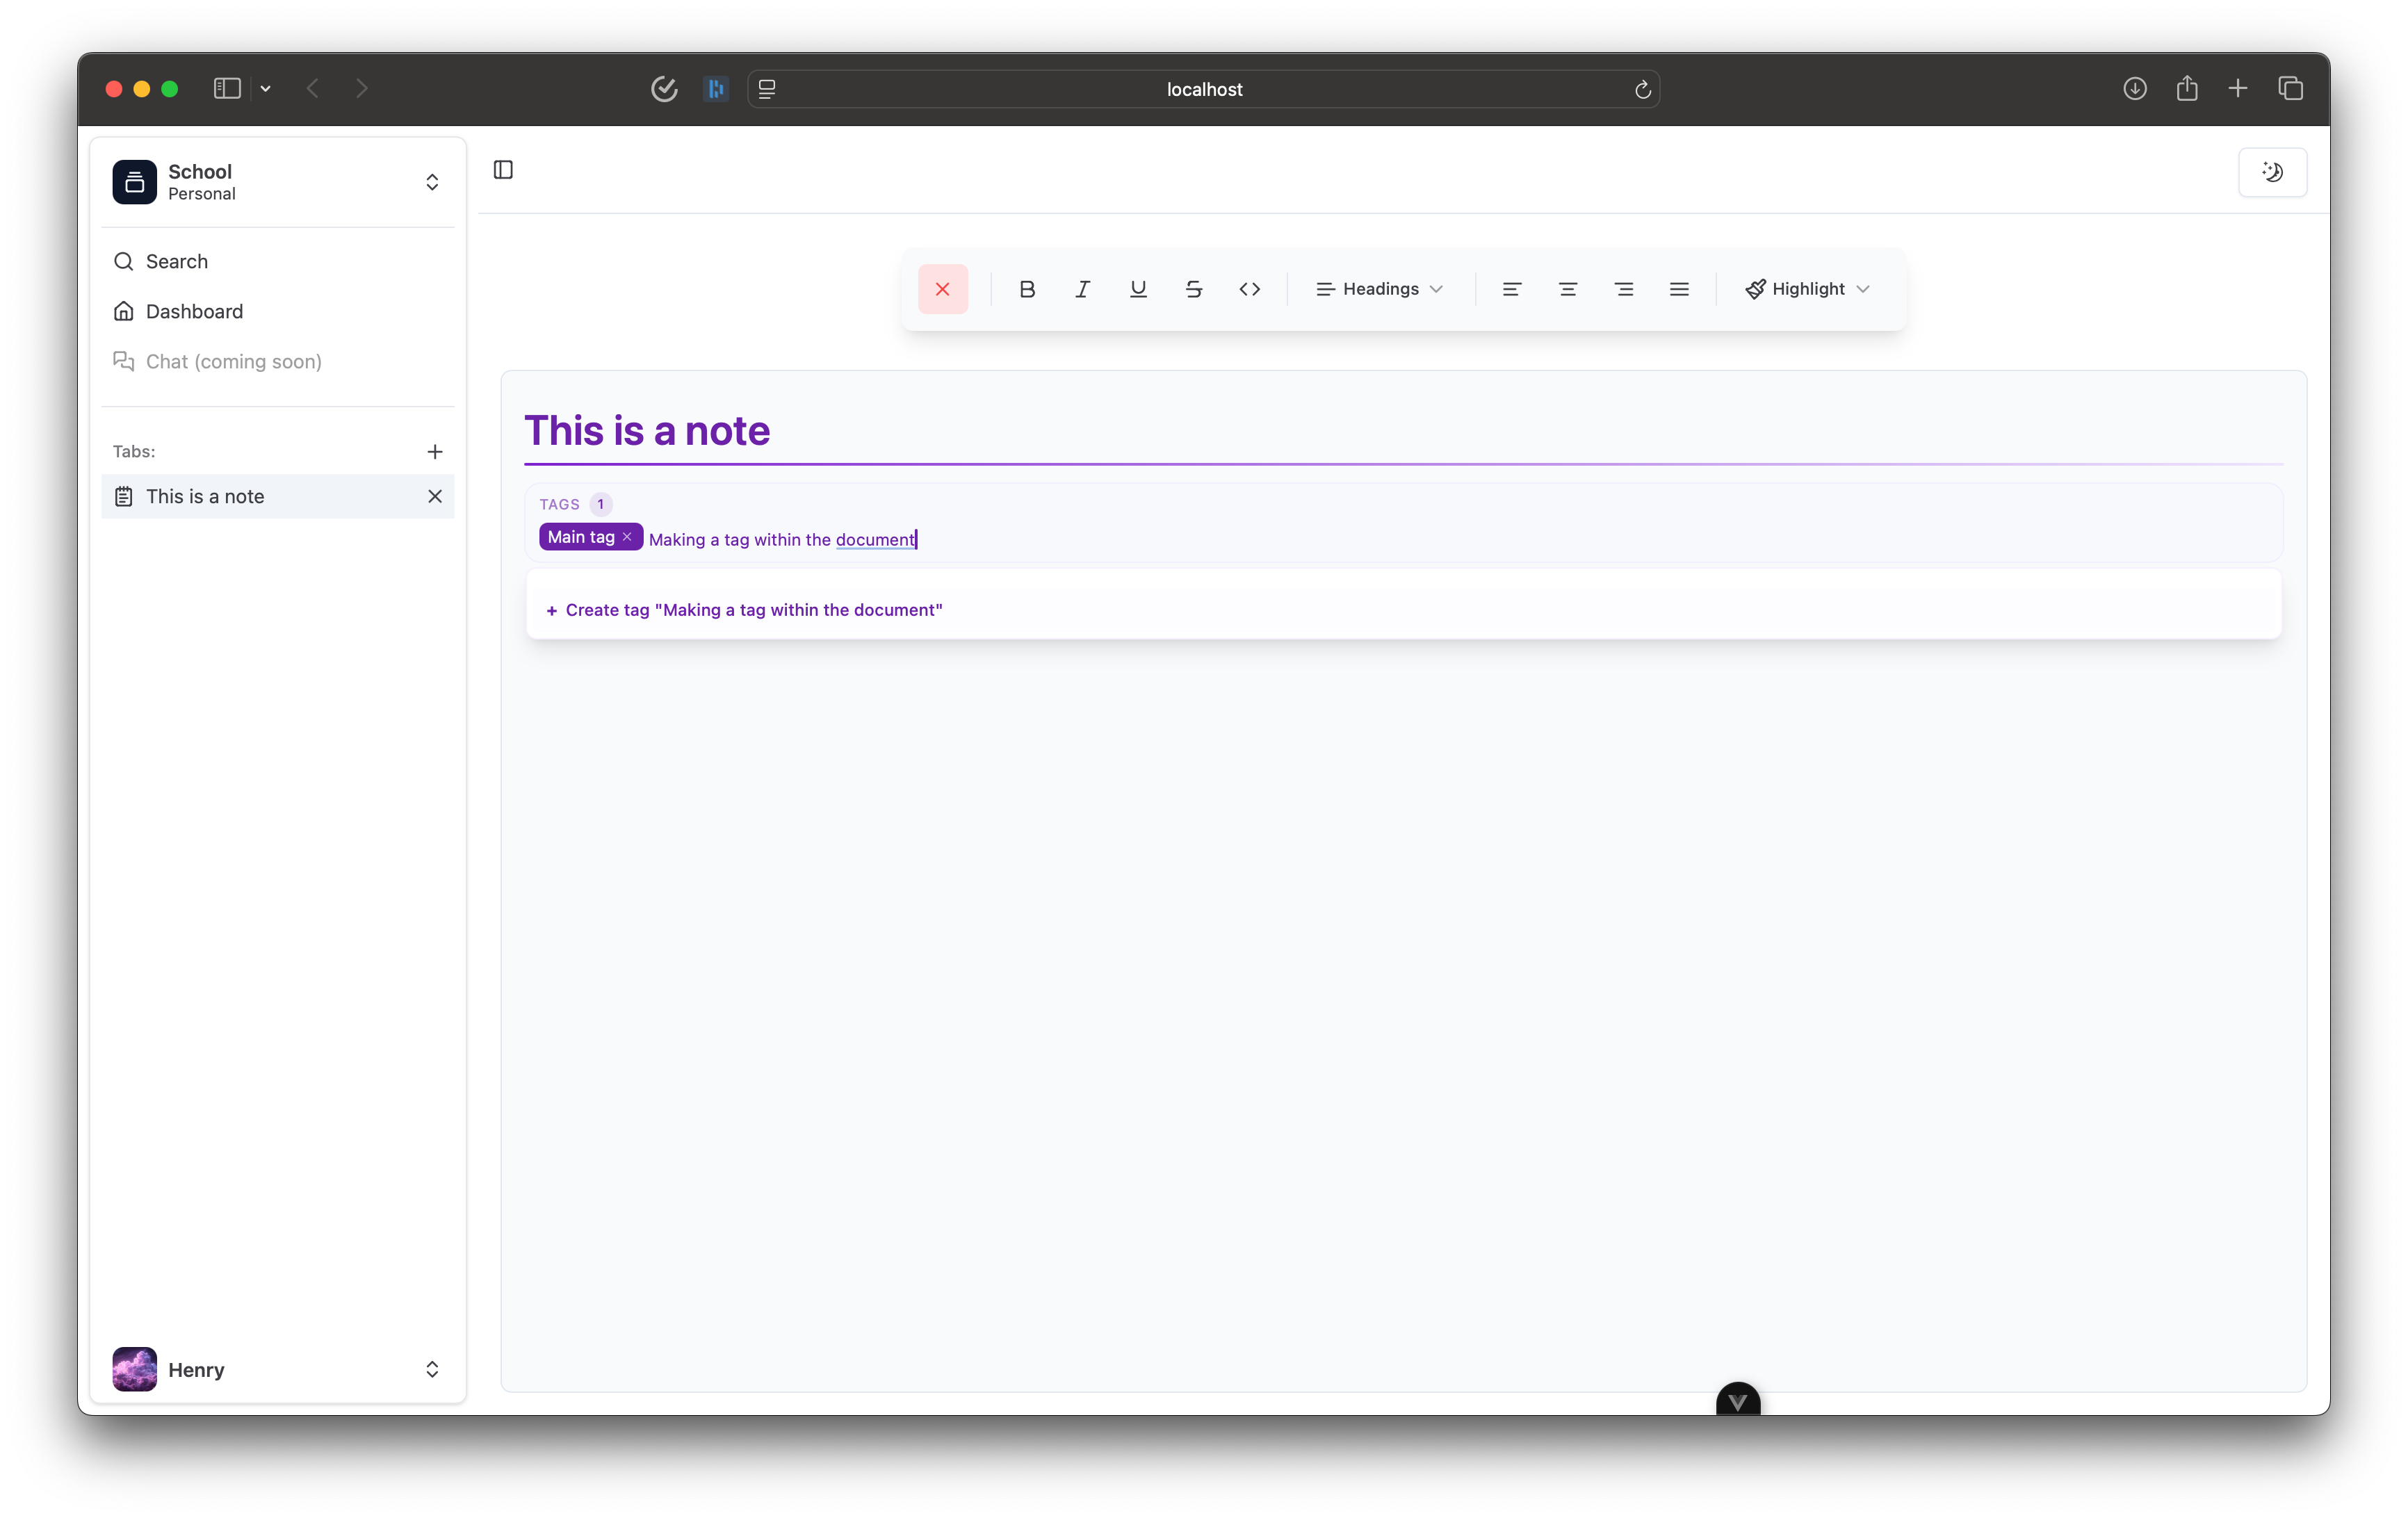
\includegraphics[width=0.8\textwidth]{Prototype/23_DocumentTagging/media/creatingTag.png}
    \caption{Creating a new tag and attaching it within a document}
    \label{fig:document_tagging}
\end{figure}

